% This is a default-selection of plugins that are used widely in this repo.

\documentclass[a4paper,10pt,fleqn]{article}
\usepackage[utf8]{inputenc}

% deutsche Trennmuster etc.
\usepackage[ngerman]{babel}
\usepackage[T1]{fontenc}

% mathematical simbols and fonts
\usepackage{mathtools} 
\usepackage{amssymb}
\usepackage{amsmath}
\usepackage{ntheorem}
\usepackage{polynom}
\usepackage{marvosym}
\usepackage{tabu}
\renewcommand*{\bmod}{\mathbin{\%}}
\everymath{\displaystyle}

\usepackage{multicol}
\usepackage{color}
\usepackage[usenames,dvipsnames]{xcolor}
\setlength{\columnsep}{1cm}
\setlength{\columnseprule}{0.25pt}
\def\columnseprulecolor{\color{gray}}
\usepackage{hyperref}

\usepackage[margin=1.5cm]{geometry}
\usepackage{graphicx}
\usepackage{pgfplots}
\pgfplotsset{compat=1.10}

%Code higlighting

\usepackage{minted}

% make lists more compact:
\newlength{\wideitemsep}
\setlength{\wideitemsep}{.5\itemsep}
\addtolength{\wideitemsep}{-5pt}
\let\olditem\item
\renewcommand{\item}{\setlength{\itemsep}{\wideitemsep}\olditem}
\renewcommand{\arraystretch}{1.25}

\title{Zusammenfassung InfSi1}
\author{Fabian Hauser}
 
\begin{document}
\maketitle

\section{Grundbegriff Sicherheit}

Sicherheit: Confidentiality, Integrity, Availability ("CIA")

\begin{description}
\item[Datensicherheit] \hfill \\
	Schutz vor Missbrauch der Daten durch organisatorische und technische Massnahmen
\item[Datenschutz] \hfill \\
	Schutz vor dem Missbrauch ihrer personenbezogenen Daten
\end{description}

\subsection{Management}
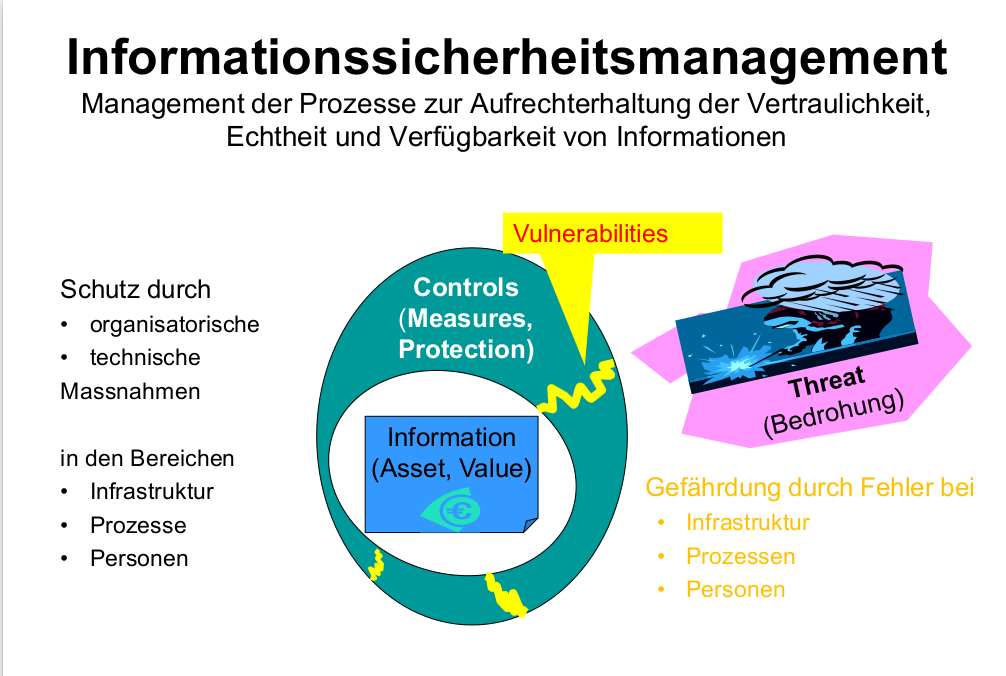
\includegraphics[scale=0.25]{img/informationssicherheitsmanagement.png}

\begin{description}
\item[Threads] \hfill \\
	Wahrscheinlichkeit eines Zwischenfalls * Schaden = Bedrohung * Verletzlichkeit * Schaden
\item[Vulnerabilities]
\item[Control] \hfill \\
	(measures, protection)
\item[Information] \hfill \\
	(asset, value)
\item[Gefährdung] \hfill \\
	(Hazard, Applied thread): Bedrohung + Schwachstelle
\end{description}


\subsection{Massnahmenkataloge}
\begin{enumerate}
\item	Infrastruktur
\item	Organisation
\item	Personal
\item	Hardware/Software
\item	Kommunikation
\item	Notfallvorsorge
\end{enumerate}

\subsection{Gefährdungskataloge (Applied Threat)}
\begin{enumerate}
\item	Höhere Gewalt
\item	Organisatorische Mängel
\item	Mengschliche Fehlhandlungen
\item	Technisches Versagen
\item	Vorsätzliche Handlungen
\end{enumerate}

\subsection{Risikomanagement}

NVD/CVE nach CVSS:	http://www.security-database.com/cvss.php


\section{Standards}

\begin{description}
\item[Formale Standards] \hfill \\
	offizielle Standards, z.B. von Internationalen Standards (ISO, IEC, ITU), Berufsverbänden(IEEE), Staatsstellen NIST
\item[Public (open) Standards] \hfill \\
	Open Source Standards (Internet RFCs)
\item[De-Facto Standards] \hfill \\
	Herzstellerspezifische Standards (z.B. MS Office, PDF, Industriestandards (DIX, ECMA)
\item[Interne Standards] \hfill \\
	(firmeninterne Standards)
\end{description}
	
\subsection{Verbindlichkeiten in Standards}
gemäss RFC 2119:

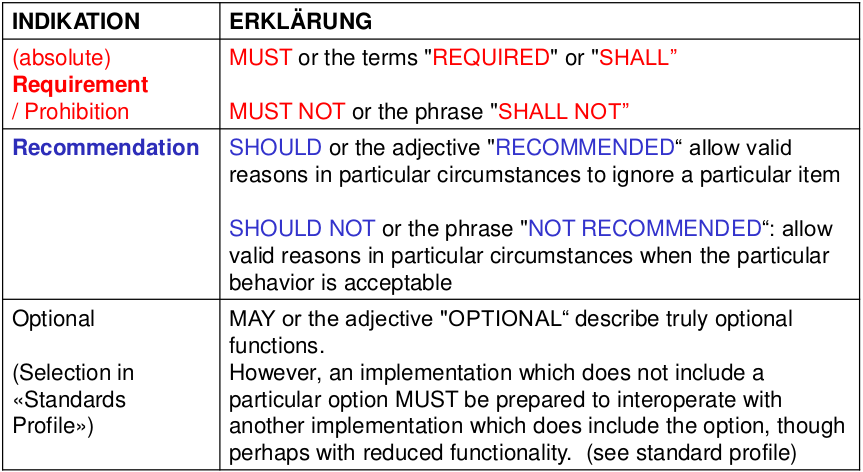
\includegraphics[scale=0.5]{img/rfc2119.png}
	
\subsection{ISO 27000}

\subsubsection{ISO 27001}
	Gibt an, was zu tun ist.
\subsubsection{ISO 27002}
	Enthält Umsetzungshinweise.

\subsection{ITIL}
	Stark angelehnt an \emph{ISO 27001}, um Sicherheit im IT Bereich zu erreichen.


\subsection{OWASP}	
	Open Web Application Security Project.
	
	Bietet Guidlines zur Verbesserung der Sicherheit von Web Applications.

\subsection{Gefährdungen}
\begin{description}
\item[Zero day exploit / attack] \hfill \\
	vulnerability that is unknown to the software vendor
\item[Spear phishing] \hfill \\
	targeted phishing to steal intellectual property, financial data, trade or military secrets and other confidential data.
\item[Advanced persistent threat (APT)] \hfill \\
	stealthy and continuous computer hacking processes, orchestrated by human(s), targeting a specific entity (organizations and/or nations) for business or political motives.
\end{description}

\subsection{Security ...}

 \begin{itemize}
 	\item Übersicht schaffen, Ziele festlegen, Checkliste/Standards nutzen
 	\item Trennung/Separierung von Systemen und Funktionen
 	\item Arbeitsanweisungen, Richtlinien, Regelungen erstellen
 	\item Ausbildung und Sensibilisierung Mitarbeiter
 	\item Kontrollen/Konsequenzen von Verstössen festlegen
 \end{itemize}

\paragraph{Objekte}
	\begin{itemize}
		\item Eigene Informationen
		\item Fremde Informationen
		\item Personen
		\item Gebäude, Räume
		\item Netze
		\item Server
	\end{itemize}

\paragraph{Grundsätzliche Prinzipien der Zugangskontrollen}

\begin{itemize}
	\item Principle of least priviledge / Need to know
	\item Same Origin Policy
	\item Sandbox
	\item Erlaubnis mit Verbotsvorbehalt (Blacklist, opt out)
	\item Verbot mit Erlaubnisvorbehalt (Whitelist, opt in)
	\item Vier-Augen-Prinzip
\end{itemize}
\end{document}


\subsection{Kryptografie}

%TODO: Formeln Wahrscheinlichkeit


\end{document}